\documentclass[12pt]{article}

\usepackage[margin=1in]{geometry}  % Set margins.
\usepackage{graphicx}              % Include graphics.
\usepackage{url}                   % Embed URLs.
\usepackage{multirow}              % Allow multi-row tables.
\usepackage{xspace}                % Add space at the end of a macro.
\usepackage{xr}                    % Allow cross-references between docs.
\usepackage[sort&compress]{natbib} % Hyphenate consecutive references.
\usepackage{setspace}

\author{Benjamin Diament\\
Department of Computer Science and Engineering\\
University of Washington\\
Seattle, WA, USA\\
bdiament@cs.washington.edu
\and
William Stafford Noble
\thanks{
to whom correspondence should be addressed.
email: william-noble@uw.edu;
phone: 206-543-4457;
fax: 206-685-7301
}\\
Department of Genome Sciences\\
Department of Computer Science and Engineering\\
University of Washington\\
Seattle, WA, USA\\
william-noble@uw.edu}

\newcommand{\XCorr}{\ensuremath{X_{Corr}}\xspace}
\newcommand{\Sp}{\ensuremath{S_p}\xspace}
\newcommand{\tidezero}{Tide-v0\xspace}



% Allow references to the supplementary tables and figures.
\externaldocument{tide-supplement}

\title{Faster SEQUEST Searching for Peptide
  Identification from Tandem Mass Spectra}

\doublespacing

\begin{document}

\maketitle

\clearpage

% 200 words maximum
\begin{abstract}

Computational analysis of mass spectra remains the bottleneck in many
proteomics experiments. SEQUEST was one of the earliest software
packages to identify peptides from mass spectra by searching a
database of known peptides. Though still popular, SEQUEST performs
slowly. Crux and TurboSEQUEST have successfully sped up SEQUEST by
adding a precomputed index to the search, but the demand for
ever-faster peptide identification software continues to grow. Tide,
introduced here, is a software program that implements the SEQUEST
algorithm for peptide identification and that achieves a dramatic
speedup over Crux and SEQUEST.  The optimization strategies detailed
here employ a combination of algorithmic and software engineering
techniques to achieve speeds up to 170 times faster than a recent
version of SEQUEST that uses indexing.  For example, on a single Xeon
CPU, Tide searches 10,000 spectra against a tryptic database of 27,499
{\it C.\ elegans} proteins at a rate of 1,550 spectra per second,
which compares favorably with a rate of 8.8 spectra per second for a
recent version of SEQUEST with index running on the same hardware.

\end{abstract}

\noindent Running title: {\sc Faster SEQUEST Searching}

% No more than 10.
\noindent Keywords: shotgun proteomics, peptide identification

\clearpage

\section{Introduction}

SEQUEST \cite{eng:approach} pioneered the pure database search
approach for analysis of tandem mass spectra from shotgun proteomics
data. Despite the passage of some time, SEQUEST remains popular: a
search on Google Scholar returns about 5,800 articles between 2006
and 2010 mentioning ``SEQUEST'' and ``peptides''.

Although SEQUEST enjoys considerable popularity, it runs slowly even
on modern architectures. Performance varies significantly based on the
size of the peptide database, and especially on the number of
candidate peptides considered per spectrum, but analysis times are
typically in the range of a second per spectrum identified.  Consequently,
efficient data
analysis of an MS/MS experiment often requires significant
computational resources, including dedicated computing
clusters. Barriers of time and expense play a correspondingly
restrictive role in experiment design. Conversely, faster
identification broadens the possibilities for experimentation.

Many approaches exist for identifying peptides from tandem mass spectra
(reviewed in reference \cite{nesvizhskii:analysis}). These methods may
be categorized broadly
as {\it de novo} methods, which analyze spectra without reference to
an external set of known peptides; database methods, which match
spectra to the closest candidate peptide in a database of known
peptides; hybrid methods, which employ some combination of the
previous two approaches; and library search methods, which compare
observed spectra to a library of previously observed, annotated
spectra.

Database search methods work by comparing each observed spectrum
against a theoretically predicted spectrum for each peptide in a
database, typically assigning a score to each database entry and
reporting the highest-scoring result. The main scoring function of
SEQUEST is \XCorr \cite{eng:approach, eng:fast}, which assigns a
similarity score to any given pairing between an observed spectrum and
the theoretical spectrum of a candidate peptide.

As originally implemented, \XCorr is costly to compute, so several
approaches have been used to improve the speed of the \XCorr
calculation. SEQUEST itself uses a faster preliminary score, \Sp,
expecting that the peptide with the highest \XCorr will also have a
sufficiently high \Sp to be included in a second scoring
round. TurboSEQUEST and Crux \cite{park:rapid} introduced to the
SEQUEST method an index
based on precursor mass to increase the efficiency of candidate
peptide retrieval.  Recently, a faster \XCorr computation,
performed as a dot product, was described in \cite{eng:fast}. This
method is included in Crux and more recent SEQUEST versions. However, despite
such advances, the need for further speed improvements remains.

In parallel to these SEQUEST-specific developments, a host of
competing database search methods have been described
\cite{perkins:probability, clauser:role, bafna:scope, zhang:probid,
  colinge:olav, tabb:myrimatch, geer:open, bern:lookup,
  roos:pepsplice, craig:tandem}, along with a variety of methods for
performing the searches efficiently.  Many of these tools use a
database index, usually indexing on precursor mass and, in one case,
also by MS/MS fragment mass \cite{tang:discovering}.  Other tools gain
efficiency by reordering the spectra themselves \cite{tabb:dbdigger}.
A variety of algorithms use {\em de novo} analysis \cite{bern:lookup},
filtering \cite{tanner:inspect}, two-pass searching
\cite{craig:tandem}, hashing \cite{dutta:speeding} or metric space
indexing \cite{ramakrishnan:fast} to efficiently reduce the effective
size of the database.  In general, such methods may perform very
effectively at the cost of losing a few identifications, or slightly
less efficiently in a lossless fashion.  Finally, some tools are
designed to exploit multi-core or multi-threaded CPUs
\cite{tabb:myrimatch}, GPUs \cite{baumgardner:fast}, clusters of CPUs
\cite{duncan:parallel} or to
make efficient use of the CPU cache \cite{roos:pepsplice, li:speeding}.  At
least one vendor, Sage-N, offers a combination hardware/software-based product.

In any database approach to peptide identification, the number of
candidate peptides may be as much as quadratic in the size of the
protein database, so all search methods must manage space
efficiently. The original SEQUEST did not include a peptide index at
all, but rather scanned the database file repeatedly for each new
peptide. This approach requires little memory and disk space, but it
runs slowly. Modern desktop computers have far more capacious memories
and disks than those from the time SEQUEST was first developed, but
memories are still typically too small to accommodate a complete
peptide list for many searches. Consequently, compression schemes such
as \cite{edwards:sequence} and \cite{edwards:novel} have been used to
reduce memory bloat.

Here, we introduce Tide, a much faster implementation of the SEQUEST
algorithm. Various versions of SEQUEST exist that differ in
detail. Tide's analysis of MS/MS spectra follows that of Crux
\cite{park:rapid}, an open source software package based on SEQUEST.
Tide yields identical \XCorr scores to those of Crux (version of
4/14/09).  However, through a combination of algorithmic enhancements,
improved system design, and better use of machine resources, Tide is
dramatically faster than recent versions of SEQUEST and Crux,
particularly when the database is created using fully enzymatic
digestion. Tide approaches space limitations by curtailing its use of
machine memory; however, Tide is not engineered toward low disk usage
because disk is typically a far cheaper resource than memory or time.
The Tide software is freely available for academic and non-profit use
as part of the Crux software toolkit
\url{http://noble.gs.washington.edu/proj/crux}.

\section{Materials and methods \label{section:methods}}

Tide is written in standard C++ including the standard template
libraries. All code is single-threaded; parallel execution is
achievable by running multiple program instances simultaneously.
During development, timing and profiling experiments were done on a
2.4 GHz Dual Pentium processor with 4 GB of memory running
Linux. Final timing measurements were performed on 2.33GHz Dual Xeon
processor with 8GB memory running Linux, with all code compiled in
64-bit mode.

Two benchmark datasets were used for both development and final
timing: a ``yeast'' set, and a larger ``worm'' set. The yeast set was
acquired on an LTQ ion trap mass spectrometer from a tryptic digest of
an unfractionated {\it S.\ cerevisiae} lysate and analyzed using a 4-h
reverse-phase separation, yielding 37,641 spectra
\cite{kall:semi-supervised}, from which 10,000 spectra were randomly
sampled. These spectra were searched against a protein database
consisting of the predicted open reading frames from {\it
  S.\ cerevisiae} (released 2004-04-02, 6298 proteins). The worm
benchmark was derived from a 24-h MudPIT analysis of {\it C.\ elegans}
proteins containing 207,804 spectra, from which 10,000 spectra were
randomly sampled.  These spectra were searched against a protein
database consisting of the predicted open reading frames from {\it
  C.\ elegans} and common contaminants (Wormpep v160, 27,499
proteins).  The spectra and databases comprising these benchmarks are
available at \url{http://noble.gs.washington.edu/proj/tide}.

Peptide indexes were generated from each benchmark protein database
for use with Tide and Crux. The indexes contained tryptic peptides of
length 6--50 amino acids and mass 200.0--7200.0 Da. These same search
parameters were applied to the SEQUEST searches. Except where noted, a
precursor mass tolerance window of $\pm3.0$ Daltons and a fully
tryptic peptide database were used in all experiments. Tide and Crux
experiments were run with full \XCorr calculation on all candidate
matches. SEQUEST experiments were run with the preliminary scoring
pass \Sp.


\section{Results}

\subsection{The SEQUEST algorithm and \XCorr}

The goal of peptide identification by database search is to label each
experimentally observed spectrum from an MS/MS run with the peptide
most likely to have generated the spectrum. Two sources of input are
examined. The first is a collection of tandem mass spectra, each
with an observed precursor mass and one or more possible charge
states. The second is a collection of protein sequences, usually
called the database, regardless of the storage mechanism.  A
successful identification of an observed spectrum as a match to a
candidate peptide sequence requires reasonable correspondence between
features of the observed spectrum and theoretically computed features
of the candidate peptide. The SEQUEST algorithm approaches the task of
peptide identification in four steps.

First, for each input spectrum to be identified, candidate peptides
are retrieved from the database, based on the precursor mass
associated with the input spectrum. The precursor mass of the observed
spectrum must match the theoretical mass of the candidate within a
user-specified tolerance, defaulting to $\pm 3.0$ Daltons. If more
than one possible charge state is given for the precursor ion, then
candidate selection is repeated for each charge state. If the database
is large, then many candidate peptides will be identified for each
input spectrum. The pairing of a single input spectrum with a single
candidate peptide is termed a {\it peptide-spectrum match} (PSM).

Next, each observed spectrum is preprocessed as follows. A set of
bins, each of width 1.0005079 Daltons, is laid over the full range of
the m/z values reported in the input file for the spectrum. Each input
MS/MS peak is bucketed into the nearest bin, which retains only the
highest intensity peak that fell into that bin. Each bin's intensity
value is then replaced with its square root. The range of bins from
lowest m/z to highest is then divided into ten equally spaced
regions. Within each region, the intensity of each bin is normalized
so that the most intense bin in every region has a value of 50. This
completes the preprocessing step performed on each spectrum.

Separately, a theoretical spectrum is computed for each candidate
peptide. The amino acid sequence, of
length $\ell$, of the candidate peptide is used to compute a
theoretical mass for each of the $\ell-1$ $b$- and $y$-ions
corresponding to all left and right substrings of the amino acid
sequence.  The theoretical mass of each of these ions is then bucketed
into bins of width 1.0005079 Daltons, just as for the observed
spectrum. The intensity of each of these $b$- and $y$-ions is given a
value of 50. Additionally, each of the following ions is computed and
bucketed to complete the theoretical spectrum:
\begin{itemize}
\item the two bins flanking each of the $b$- and $y$-ions each with
  intensity 25,
\item a peak with intensity 10 representing the neutral loss of
  ammonia from each $b$- and $y$-ion,
\item a peak with intensity 10 representing the neutral loss of water
  from each $b$-ion, and
\item each $a$-ion, with intensity 10.
\end{itemize}
For spectra with precursor charge of 3 or higher, doubly-charged versions of
each of the above ions are included in the theoretical spectrum.

The last step in the SEQUEST algorithm is to compare the preprocessed
observed spectrum and candidate theoretical spectrum for each
peptide-spectrum match. Preprocessing of an observed spectrum or
generating a theoretical spectrum for a candidate peptide yields
a peak-intensity vector, any pair of which may be compared. After a
spectrum is processed to obtain a length-$N$ vector $u$ and a candidate
match's theoretical spectrum is computed to get another vector $v$,
where $N$ is the number of bins, the following function is computed to
obtain the \XCorr as the score for the peptide-spectrum match:
\[\XCorr(u,v)=\langle u,v\rangle-\frac{1}{150}\sum_{\tau=-75}^{75}{\sum_{i=1}^{N}{v_iu_{i-\tau}}}\]
For each spectrum, the PSM with the highest \XCorr scores is output
to the user.

SEQUEST mitigates the slowness of computing \XCorr for every PSM by
computing an approximate preliminary score (\Sp) for each
peptide-spectrum match that it collects; only the 500 highest scoring
candidates by \Sp are fully scored by \XCorr. Tide does not compute
\Sp because it is able fully to compute \XCorr extremely
efficiently; computing \Sp as a preliminary score would not be
expected to improve Tide's speed.

For most applications, the database of proteins, from which candidate
peptides are derived, is considered to change infrequently. As a
consequence, an arbitrary amount of precomputation may be performed on
the peptide set before input spectra are to be analyzed.  Several
recently developed search tools, including TurboSEQUEST, Crux and
Tide, take advantage of this opportunity by indexing the peptide set
by precursor mass ahead of time.

Crux, Tide and various versions of SEQUEST all implement the
algorithm above, but there are some differences among them. Crux's
scoring is not identical to SEQUEST, though it is similar; see
\cite{park:rapid} for a comparison of Crux and an early version of
SEQUEST.

Through successive optimizations, a consistent aim of Tide was very
precise fidelity to Crux's results and \XCorr computation, though
Crux, in turn, adhered more loosely to SEQUEST. Tide's scoring is
identical to Crux's when Crux is compiled with double-precision
floating-point arithmetic. Figure~\ref{figure:scatter} compares
the \XCorr scores computed by Tide against those computed by two
different versions of SEQUEST. These scoring differences between Tide
and SEQUEST are no bigger than those between the two SEQUEST versions,
which are compared at the bottom of the figure.

%\subsection{Post-translational Modifications}

Tide supports searching databases with variable post-translational
modifications (PTMs). At indexing time, the user may indicate a list
of possible PTMs to include in the index. The user specifies each
variable modification as a triple: a limit on the number of
occurrences per peptide, a set of amino acids that are subject to the
modification, and the corresponding mass.  Multiple variable
modification types may be specified. For example, the specification
``2M+16.0, 5STY+79.97'' indicates that up to two occurrences of
methionine may be oxidized and up to five occurrences of any residues
serine, threonine, or tyrosine may be phosphorylated. Peptides that
are subject to the indicated variable modifications will appear in the
database multiple times, reflecting the various modified forms.

In both SEQUEST and Tide, including PTMs increases the number of
candidate peptides exponentially in the number of modifiable amino
acids per peptide.  As with SEQUEST and other database search engines,
the user is encouraged to use variable modification search judiciously
so as not to create large numbers of false positive matches or
increase search times exponentially. Tide scores a match with a
modified peptide exactly as it would the unmodified peptide, except
that it accounts for the change in mass of the modified residues.

\subsection{Baseline version of Tide \label{subsection:tidezero}}

An initial rewrite of the search method of Crux, called \tidezero, was
produced with the goal of precisely matching the \XCorr scores
produced by Crux, but with a greatly simplified code base, more easily
amenable to human analysis, machine timing and profiling, and staged
optimizations.  \tidezero served as a starting point for the
sequential introduction of a series of optimizations described in
Section~\ref{subsection:optimizations}. The operation of \tidezero was as
follows, schematized by the data flow in Figure~\ref{figure:dataflow}(A).

\begin{figure}
\centering
\begin{tabular}{cc}
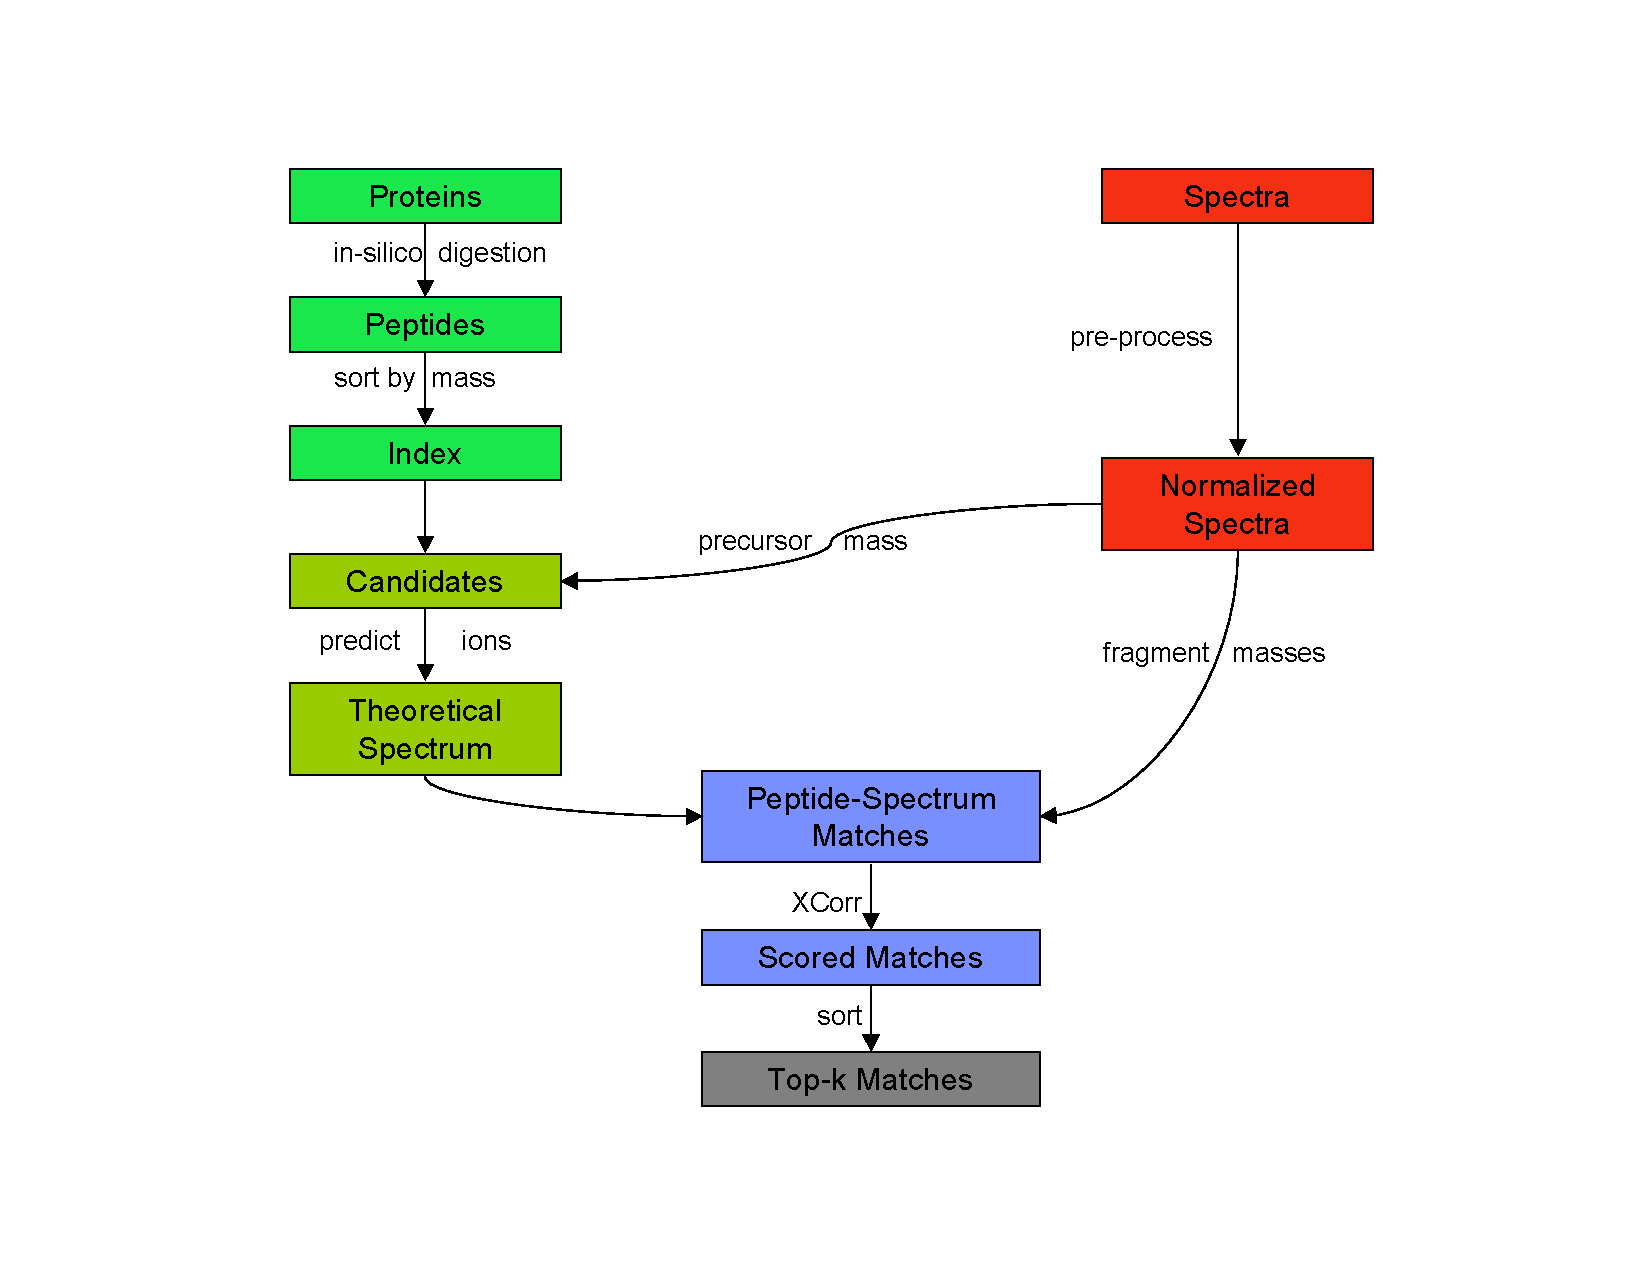
\includegraphics[width=3.0in]{Diagrams_p1-p1-cropped.pdf} &
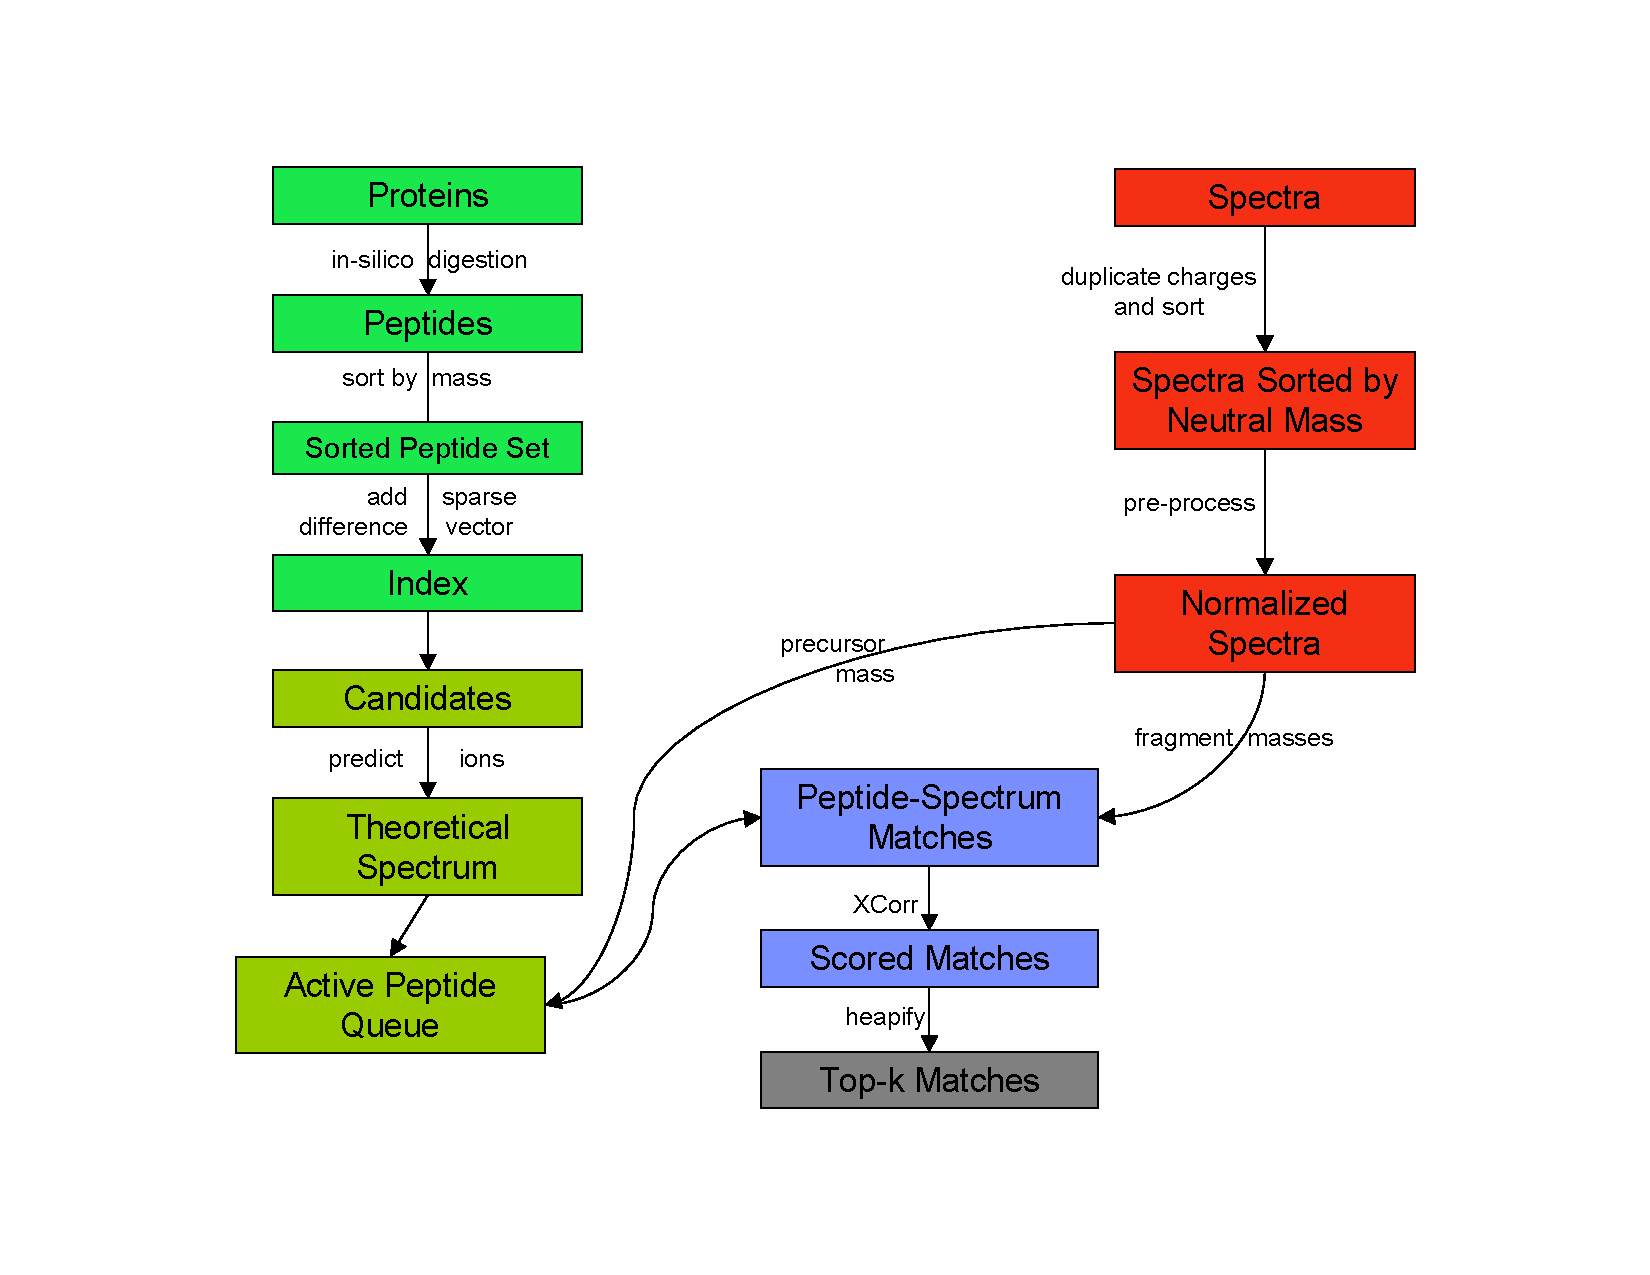
\includegraphics[width=3.0in]{Diagrams_p2-p2-cropped.pdf} \\
(A) Before & (B) After \\
\end{tabular}
\caption{{\bf Data flow in Tide before and after optimization.}
  \label{figure:dataflow}}
\end{figure}

The left side shows the progression from a protein set, supplied as a
FASTA file, to a set of peptides, to a set of theoretical
spectra. Each of these datasets is computed in turn from its parent
dataset in the diagram. The computational digestion of the proteins
and the ordering of the peptides are precomputed during an indexing
phase that needs to be run only once for a given protein database.
During the indexing phase, each protein in the input FASTA file is
computationally digested into peptides according to user-specified
parameters, which may specify enzyme and minimum and maximum peptide
sizes.

The right side of the figure shows the set of observed spectra,
including precursor $m/z$ and possible charge states, which are input
at search time. As each spectrum is considered in turn, candidate
peptides are identified, based on precursor mass, from the precomputed
index, and a theoretical spectrum is calculated for each
candidate. The bottom of the figure shows the observed spectra and
theoretical spectra matched by precursor mass, then scored by
\XCorr. For spectra with multiple possible charge states, Tide simply
iterates over each such state and considers it in turn.


\subsection{A series of optimizations \label{subsection:optimizations}}

We now briefly describe the successive algorithmic optimizations and
techniques incorporated in Tide, showing the course of development
from \tidezero to the current version of Tide. The reader interested
in more detailed descriptions of the individual optimizations should
refer to the supplementary material.

\begin{itemize}

\item {\bf Sparse representation of theoretical peaks} Each peptide's
  theoretical spectrum consists of ten peaks for each amino acid in
  the peptide, for each charge state, corresponding to the major ion
  types and the related neutral losses. Since there are roughly 1,000
  mass/charge buckets (depending on machine settings), and since most
  peptides are short (under 20 amino acids), the theoretical spectrum
  is typically sparse, so Tide uses a sparse representation of the
  theoretical peaks. This change enabled another technique---making
  theoretical peaks five-fold sparser.

\item {\bf Heapify to find top matches} As Crux finds candidate
  peptide-spectrum matches, it adds them to an array, which it sorts
  to find the best five matches. In place of this sort, Tide uses a
  heapify operation which requires linear time rather than the $O(n
  \log(n))$ time required by the sort to find the top matches.

\item {\bf Linearizing background subtraction} Tide linearizes the
  double loop that calculates \XCorr, as described in the supplement.
  At the stage it was introduced, this speedup reduced the total
  running time by about 47\% (see line 5 in Table~\ref{table:timing}).

\item {\bf Caching multiplications} The \XCorr calculation requires
  computing a dot product between the observed spectrum with each
  candidate theoretical spectrum.  Tide exploits the fact that the
  theoretical peaks may have one of only three possible intensities:
  10, 25 or 50.  A simple caching scheme thereby allows for the
  elimination of multiplications during the dot product computation.

\item {\bf Join with rolling window} Before any matching begins, Tide
  reads the observed spectra into memory and sorts them by mass.  In
  case a spectrum has multiple possible charge states it appears in
  the sorted array once for each charge state, as the join is
  performed on the neutral (uncharged) mass.  After the spectra are
  sorted, Tide iterates in parallel over the spectra and the
  presorted candidate peptides.  Iteration in this fashion creates a
  ``rolling window,'' which occupies only as much memory as is
  required to store a window's worth of theoretical spectra. This
  strategy, which is illustrated in Figure~\ref{figure:dataflow}(B),
  enables reuse of the computation of the theoretical spectra so that
  no theoretical spectrum need ever be computed more than once.

\item {\bf Making the theoretical peaks vector five-fold sparser}
  Theoretical spectra in the SEQUEST algorithm occur in groups
  corresponding to cleavage events, with somewhat predictable spacing
  among the peaks within a group. Tide takes advantage of such peak
  groupings to represent the complete set of theoretical peaks even
  more sparsely. This is done by adding together the peaks in a group
  as part of the spectrum preprocessing step. Details are given in
  Section~\ref{subsubsection:fivefold} of the supplement.

\item {\bf Fixed point arithmetic} Rather than compute the dot product
  in double-precision floating-point arithmetic, Tide uses fixed-point
  arithmetic. To do this, Tide multiplies each entry in the spectrum
  by a large constant ($10^7$) and rounds to the nearest integer. The
  constraints imposed by the normalization procedure ensure against
  underflow or overflow, and the fact that the dot product is a simple
  summation assures numerical stability. We therefore achieve the same
  results as Crux does to at least five or six decimal places.

\item {\bf FIFO memory allocator} Profiling of a larger dataset showed
  that significant time was being spent in memory heap operations,
  many of which were tied to allocating and deallocating space for
  theoretical spectra and associated data. Therefore, Tide includes a
  specialized first-in-first-out (FIFO) memory allocator that performs
  well on data associated with a queue.

\item {\bf Compiled dot-product code} Following the above speed
  improvements, profiling revealed that most of the remaining time
  (about $60\%$) was spent in the dot product computation.  Although
  this code had already been optimized twice---using cache lookups
  instead of multiplication operations, and using two such lookups
  rather than three---testing still showed that unrolling the loop
  and hard-coding specific values for the array of theoretical peaks
  was about twice as fast.  To take advantage of this opportunity,
  Tide performs a run-time compilation for each theoretical spectrum
  to {\tt x86} machine code to execute the sum with preset values. The
  appropriate code is generated in a buffer for each candidate
  peptide, and the program is instructed to jump to the buffer to run
  this peptide-specific dot-product code.

\end{itemize}

\begin{table}
\centering

\begin{tabular}{|r|l|p{0.43\textwidth}|r|r|p{0.7in}|}
\hline
\multicolumn{1}{|c|}{} & \multicolumn{1}{|c|}{Text} & \multicolumn{1}{|c|}{Description} & \multicolumn{1}{|c|}{Worm} & \multicolumn{1}{|c|}{Yeast} & \multicolumn{1}{|c|}{\% Change} \\
\hline
1 & & Crux baseline (4/14/09) & 5:47:37.9 & 36:03.5 &  \\
\hline
2 & \S\ref{subsection:tidezero}, \S\ref{subsection:optimizations} & Rewrite including deduplication of peptides; heapify; compressed peptides file; and eliminating seeks. & 7:39.0 & 2:41.6 & 45.4-fold reduction  \\
\hline
3 & {\S}S\ref{subsubsection:sparsepeaks} & Sparse representation of theoretical peaks. [Note that input file parsing is introduced here, and removed later.] &  & 1:50.5 & -31.6\% \\
\hline
4 & & Fixed-capacity arrays for theoretical peaks; better memory management. &  & 1:13.4 & -33.3\% \\
\hline
5 & {\S}S\ref{subsubsection:linearize-bkgnd-sub} & Linearizing the background subtraction for \XCorr computation. &  & 0:38.9 & -47.2\% \\
\hline
6 & {\S}S\ref{subsubsection:join} & Active peptide queue and sorted spectra (rolling window join). & 0:38.8 & 0:13.8 & -64.5\% \\
\hline
7 & \S\ref{subsection:optimizations} & Eliminate input file parsing. [See text; and compare line 3 above.] & 0:25.6 &  & -22.2\% \\
\hline
8 & & Omit calculation with theoretical ions outside spectrometer's range. & 0:23.7 &  & -7.4\% \\
\hline
9 & {\S}S\ref{subsubsection:fivefold} & Sparse difference vector representation. & 0:24.7 & 0:09.0 & 4.2\% \\
\hline
10 & {\S}S\ref{subsubsection:striping} & Array striping to eliminate one lookup during dot product calculation. & 0:20.4 &  & -17.4\% \\
\hline
11 & {\S}S\ref{subsubsection:fivefold} & Store the vector diffs to disk instead of calculating at runtime. & 0:15.5 & 0:05.9 & -24.0\% \\
\hline
12 & {\S}S\ref{subsubsection:fixedpoint} & Fixed-point arithmetic. & 0:14.7 & 0:06.0 & -5.2\% \\
\hline
13 & {\S}S\ref{subsubsection:fifo}, {\S}S\ref{subsubsection:compiler} & FIFO memory allocator and run-time compiled dot-product code. & 0:8.6 & 0:4.4 & -34\% \\
\hline
\end{tabular}

\caption{{\bf Wall clock time after successive optimizations.}
  Optimizations in the order they were introduced into Tide, and the
  measured improvement introduced by each. In several cases, earlier
  optimizations were prerequisite for later ones: e.g. line 9 showed a
  slight degradation, but was prerequisite for the gain in line
  11. Where indicated, the reader is referred to a section of the text
  or supplement (section numbers preceded by S) for details.  These
  measurements, taken during Tide's development, were done on a
  different machine than the one used for final timing measurements
  (see Section~\ref{section:methods}).
  \label{table:timing}}
\end{table}

\begin{figure}
\centering
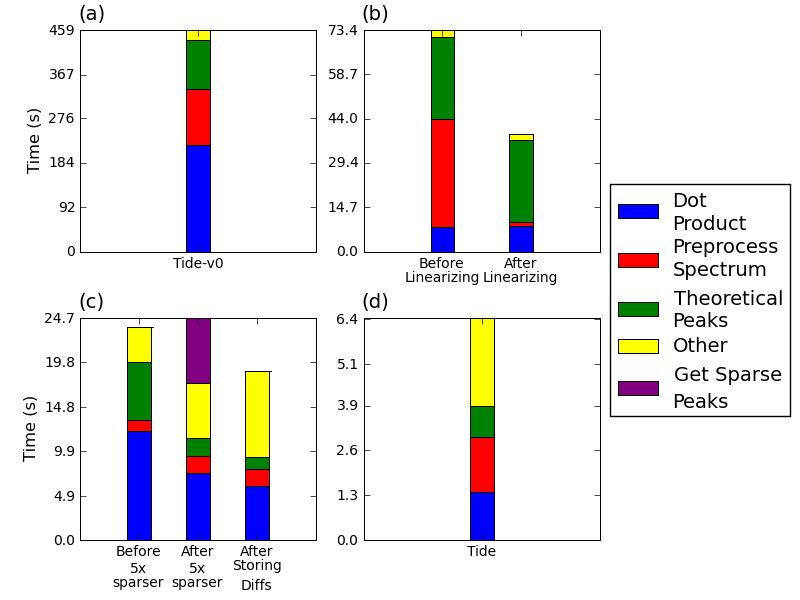
\includegraphics[width=6.0in]{profiles.png}
\caption{{\bf Profile of various development stages of Tide} for the worm
  benchmark (10,000 spectra).  Each profile shows how much computing
  time was spent in each of the major phases of Tide's operation at
  various points during development.  Such profiles aided in deciding
  how best to proceed with optimization efforts. Profiles shown are
  (a) \tidezero; (b) before and after linearizing background
  subtraction (Supplement
  Section~\ref{subsubsection:linearize-bkgnd-sub}); (c) before and
  after fivefold sparser representation, and after storing $d$ to disk
  (Supplement Section~\ref{subsubsection:fivefold}); and (d) the
  current version of Tide. For each plot, the (diminishing) total
  execution time is indicated via the y-axis scale.
  \label{figure:profiles}}
\end{figure}

Table~\ref{table:timing} shows timing results in the actual order
these changes were introduced to Tide, with later optimizations often
building upon earlier ones. Each line shows the performance change
following the incorporation of perhaps a few changes at a
time. Figure~\ref{figure:profiles} shows the profile of major program
components at various key points along the way.

The following features of the timing table bear some further
exposition. The earliest working version of Tide shows a 45-fold
improvement over the run-time of Crux. A substantial portion of this
dramatic improvement likely reflects artifactual slowness of Crux that
happened to be present at the time Tide got under way, and was since
corrected in Crux. Newer versions of Crux, such as the one used for final
timing measurements, are much faster.

Artifacts, however, do not completely account for the dramatic 45-fold
speedup of \tidezero over Crux. The 3-Dalton mass window and full
\XCorr scoring for all candidates are settings for which Crux may not
have been optimized, and they are time-consuming settings. Tide's code
was also a lot more compact at this point (about 1,200 lines, compared
to Crux's $\sim$32,000), and perhaps mere removal of some code complexity
helped this initial number. The initial version of Tide also
implemented heapify, described below; it used a compressed peptide
file that holds pointers to all the proteins in which it is found; and
it managed for these datasets to read all the compressed peptides into
memory, eliminating most disk seeks. All these changes contributed to
the immediate gains over Crux, but no separate measurements were made
for each of these improvements. Versions of Tide from
Table~\ref{table:timing} line 6 onward do not require the index to fit
into memory.

About midway through Tide's development, parsing of the input file
was jettisoned, and the input spectra were represented by an
uncompressed binary file. This was done because the particular input
file format is incidental to the main search algorithms, there are
many input file formats available, and optimizing the ms2 format in
particular fell outside the scope of efforts on Tide. The timing
numbers in two lines of Table~\ref{table:timing} reflect this
decision: Line 3 includes the parsing for the first time (a binary
file was used beforehand), and Line 7 removes it again.

The sparse difference vector representation, shown in line 9 of
Table~\ref{table:timing}, introduced a slight time penalty, but was implemented
as a prerequisite for storing the sparse vector differences to disk (line 11 of
Table~\ref{table:timing}). The two changes taken together performed very well.

Note also that running times were not always collected for both yeast
and worm, as a profile of one or the other was often enough to discern
where to focus effort; but at least one or the other time is always
reported, as is the relative time improvement between versions. An
average is shown in cases where both yeast and worm times were
measured.

\subsection{Final timing comparisons}

\begin{figure}
\centering
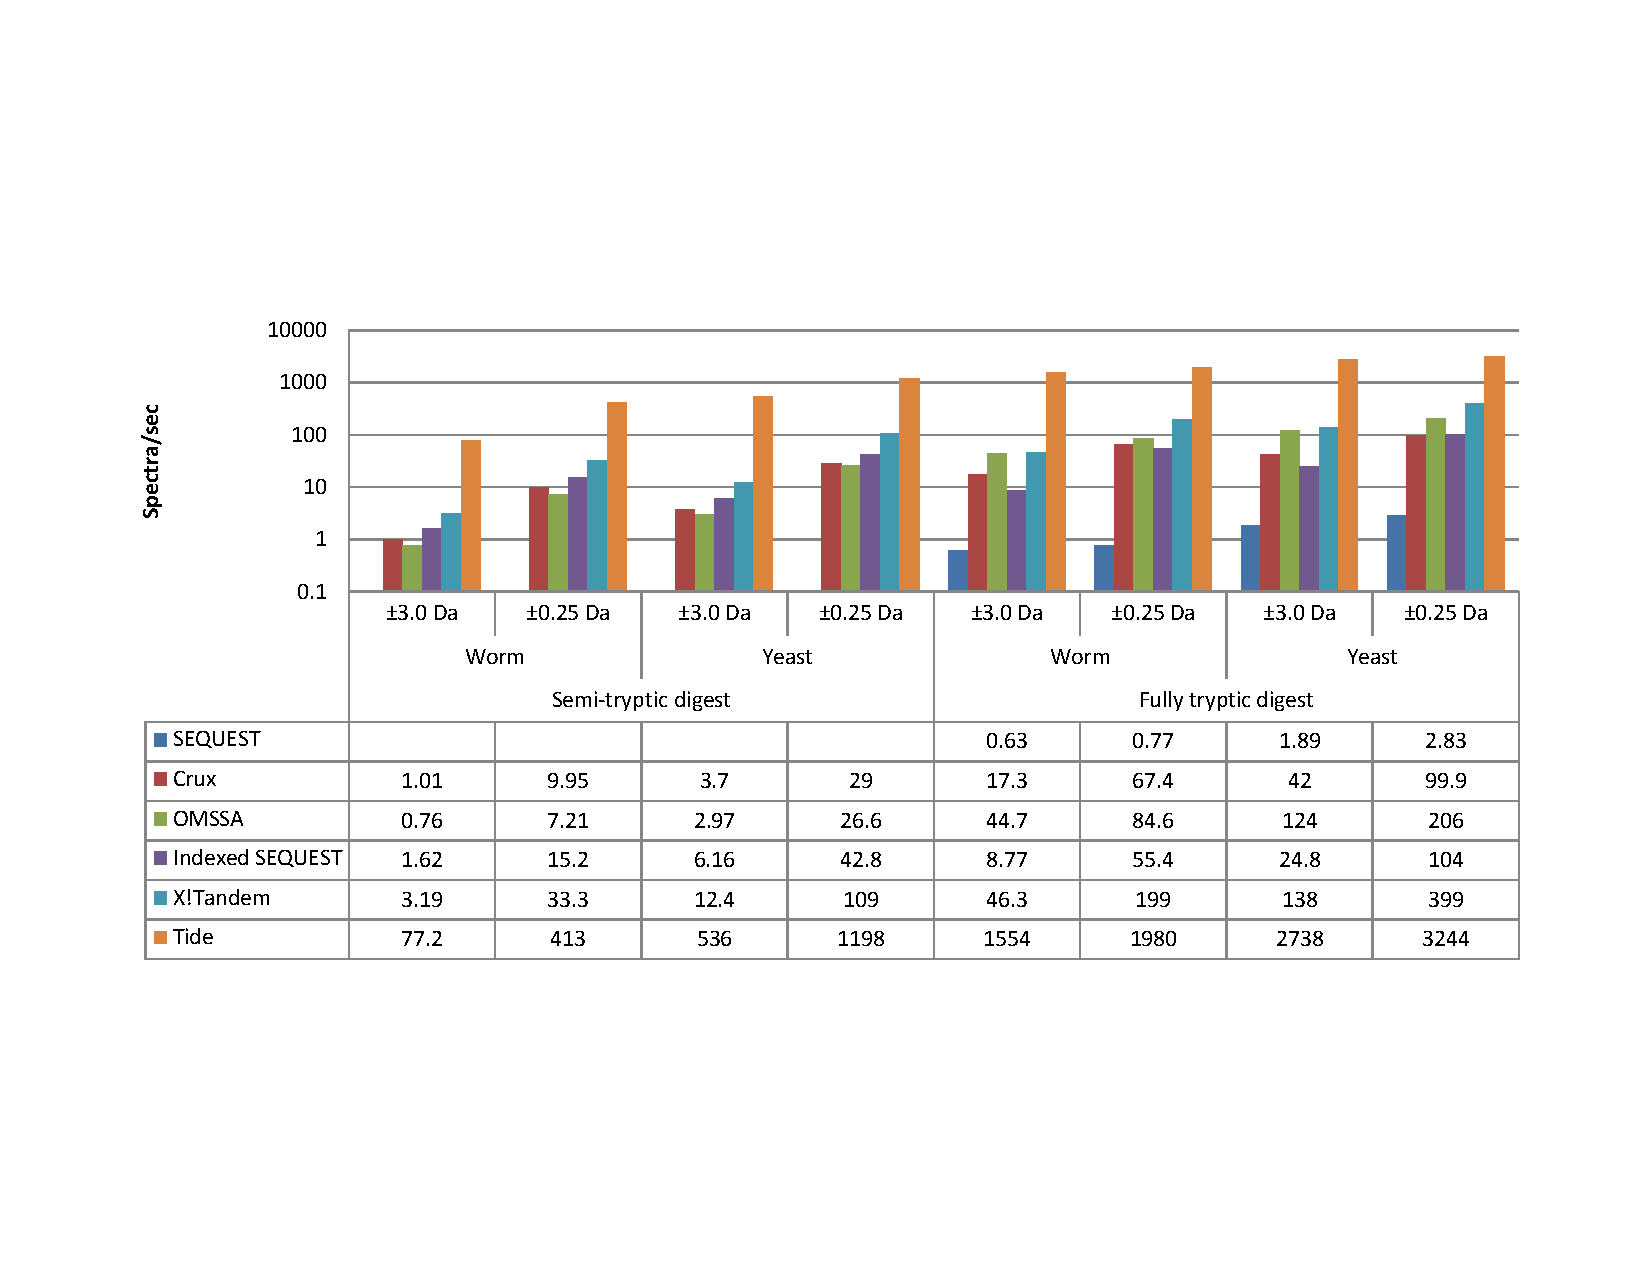
\includegraphics[width=6.5in]{timing_chart_main-cropped.pdf}
\caption{Performance of Tide compared to SEQUEST, Crux, OMSSA, Indexed
  SEQUEST (11/2009), and X!Tandem. Performance was measured in eight
  settings, varying the percursor mass tolerance window, the digest
  (fully tryptic candidate peptides or semi-tryptic), and the dataset
  ({\it C. elegans}, ``worm dataset'' or {\it S. cerevisiae}, ``yeast
  dataset''---see Methods). Bar heights in log scale show
  spectra processed per second, with numerical results given
  below. Each experiment was repeated at least 3 times with average
  timings shown, except for the X!Tandem experiments. Because SEQUEST
  runs relatively slowly, all SEQUEST
  experiments, as well as Crux experiments using semi-tryptic digestion,
  were performed with 100 randomly-selected spectra. The remaining
  experiments, including all Tide experiments, were performed using
  10,000 benchmark spectra.
  \label{figure:perf-chart}}
\end{figure}

Figure~\ref{figure:perf-chart} shows the results of timing experiments
for two SEQUEST versions, Crux, and Tide, performed on the benchmark
datasets.  For reference, timing comparisons are shown to X!Tandem and
to OMSSA, although these software packages use different scoring
methods than the SEQUEST method.

Compared to the earlier version of SEQUEST (version 2.8, 1999), Tide's
speedup is over 1,000-fold in all cases, reaching as high as
2,500-fold for the worm benchmark with fully tryptic digestion. The
increase is more modest, but still dramatic, with respect to the
recent SEQUEST version (November 2009), especially with respect to
semi-tryptic digestion---as little as 27-fold speedup for the worm set with
0.25~Da mass tolerance. The geometric average speedup for all
datasets of Tide over the recent SEQUEST build is 54-fold. The earlier
version of SEQUEST (1999) did not support semi-tryptic enzyme digestion,
and corresponding entries are blank in Figure~\ref{figure:perf-chart}.

Crux shows intermediate performance between that of SEQUEST and
Tide. Tide ran at least 29-fold faster than Crux in all cases, and as
high as 145-fold in the case of the yeast benchmark with semi-tryptic
digestion and a $\pm 3.0$ Dalton precursor tolerance. With respect to
the original SEQUEST version, Crux was as much as 87 times faster
(worm benchmark, full digestion, 0.25-Dalton tolerance). In comparison
to the recent indexed version of SEQUEST, Crux's performance was
mixed, with Crux performing faster on three benchmarks and indexed
SEQUEST performing faster in five. However, in no case was the
performance difference between Crux and the recent SEQUEST more than a
factor of two.

Although Tide performs very well in comparison to X!Tandem and OMSSA
(a geometric average of 17 times faster than X!Tandem and 43 times
faster than OMSSA over all the benchmark datasets), marked differences
in scoring methods among these systems make fair comparisons difficult
and are beyond the scope of this paper.

Four of the software packages discussed here make use of indexing to
achieve fast execution.  However, the relative speeds of three of
these tools---indexed SEQUEST, Crux and X!Tandem---fall within a
relatively narrow range of one another, spanning an average (geometric
mean over all benchmarks) factor of 4 from the slowest to the
fastest. Thus, Tide's achievement of a further 17-fold over the
fastest of these methods is especially noteworthy.

\begin{figure}
\centering
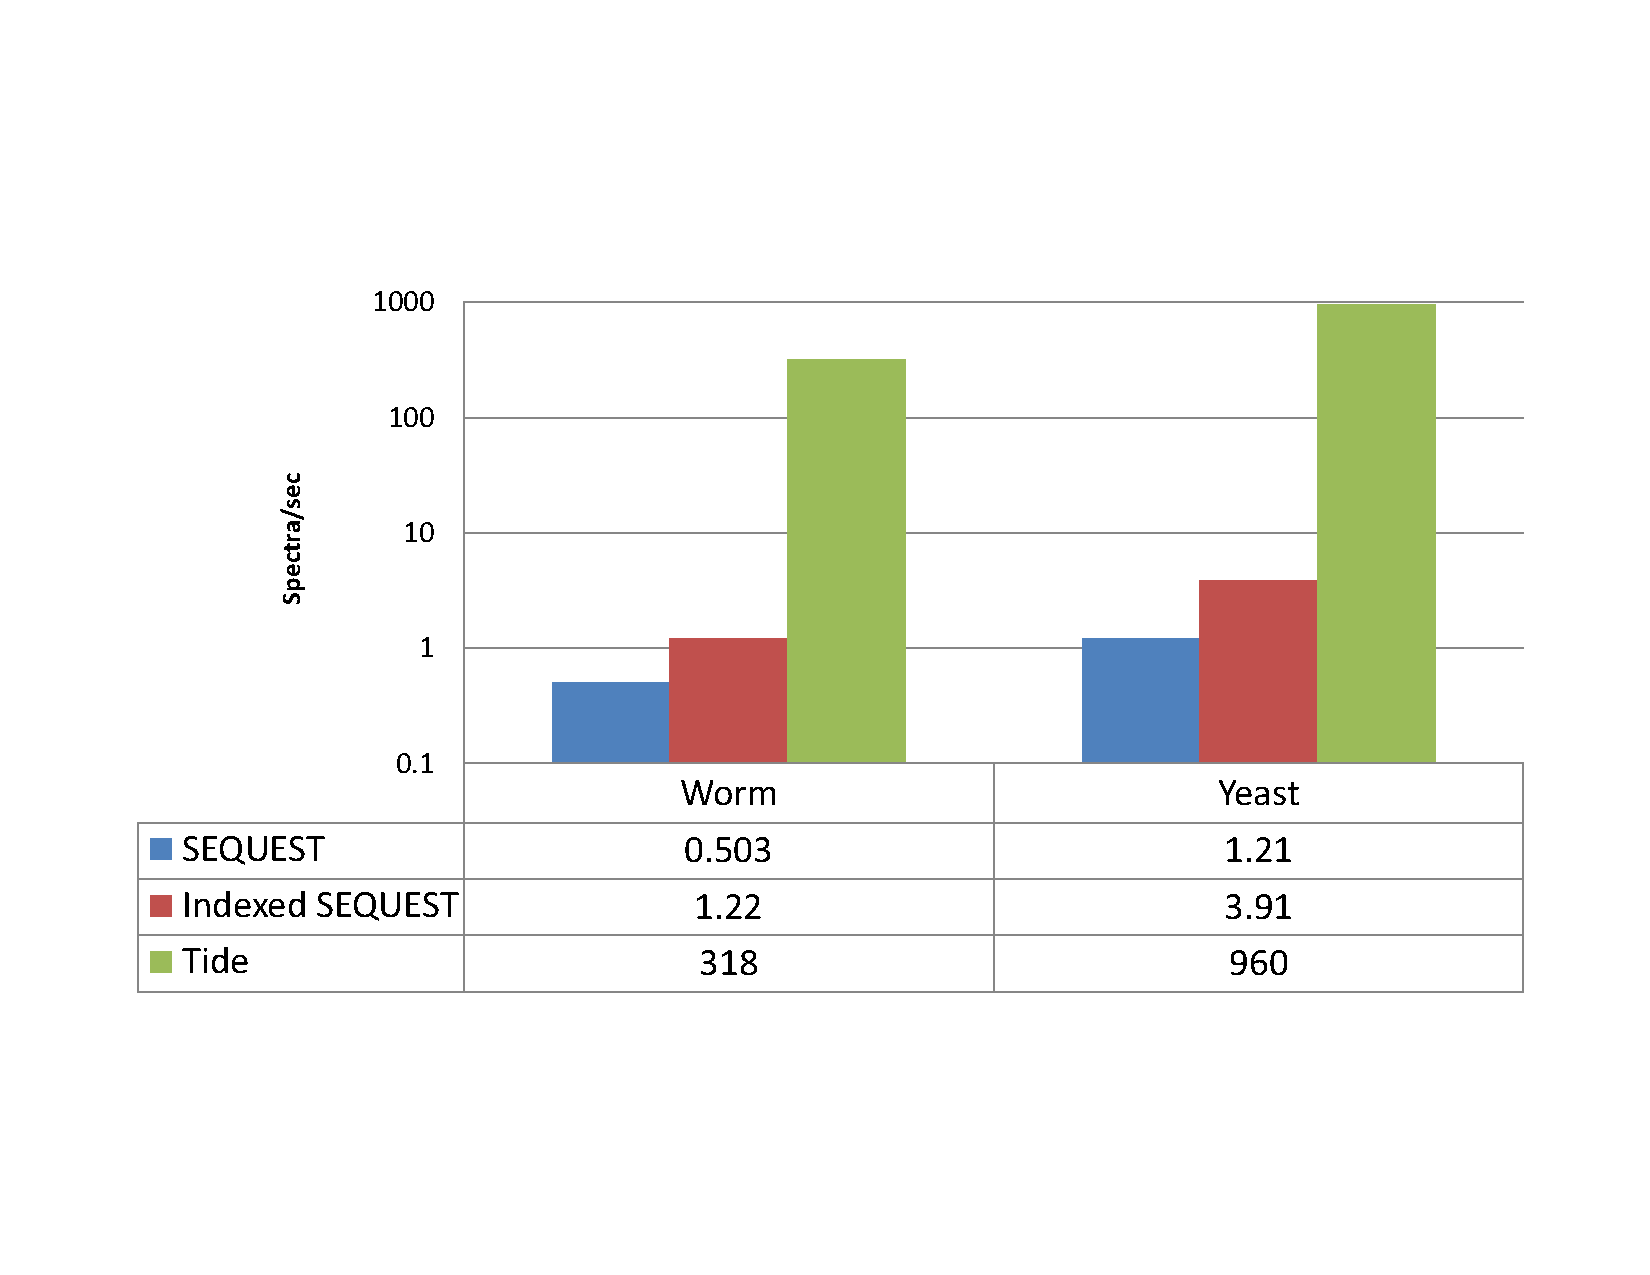
\includegraphics[width=6.5in]{timing_chart_mods-cropped.pdf}
\caption{Performance of Tide compared to SEQUEST and Indexed SEQUEST
  (11/2009) on benchmark datasets with variable modifications. Bar
  heights in log scale show the number of spectra processed per
  second.  The same benchmark datasets were used as in
  Figure~\ref{figure:perf-chart}, but with up to two occurrences per
  peptide of phosphorylated residues serine, threonine, or
  tyrosine. Tests were run with a $\pm3.0$ Dalton mass window and full
  tryptic digestion. As in Figure~\ref{figure:perf-chart}, SEQUEST
  experiments were run with 100 randomly-selected spectra, whereas Tide
  experiments used 10,000 benchmark spectra.
  \label{figure:perf-chart-mods}}
\end{figure}

\begin{figure}
\centering
\begin{tabular}{cc}
Yeast & Worm \\
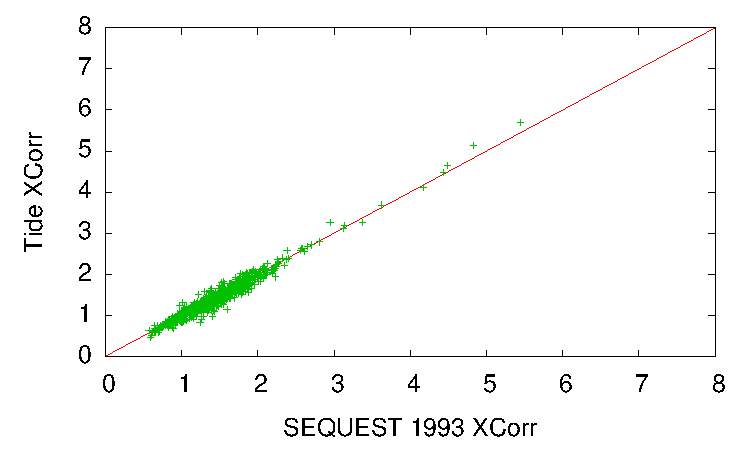
\includegraphics[width=3in]{scatter/xcorr_xcorr_yeast_seqorig_tide.pdf} &
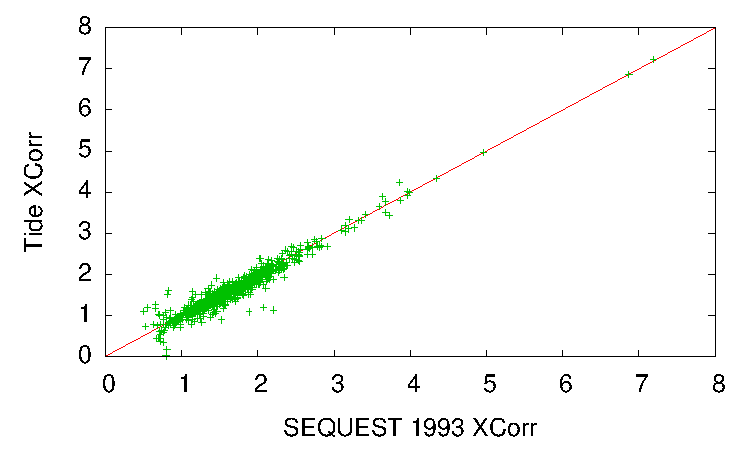
\includegraphics[width=3in]{scatter/xcorr_xcorr_worm_seqorig_tide.pdf} \\
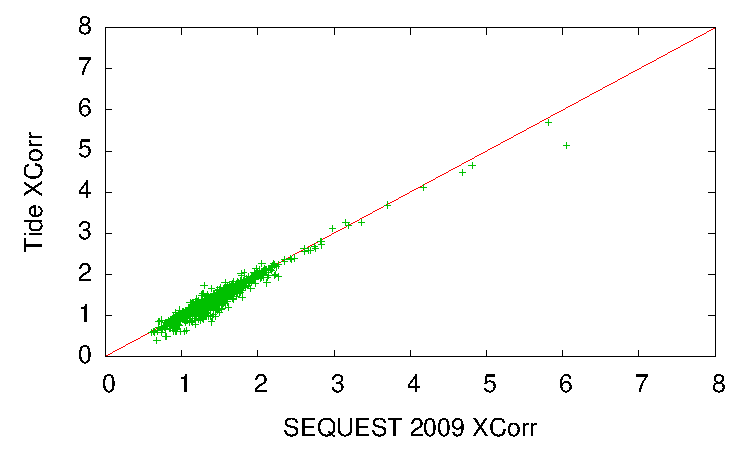
\includegraphics[width=3in]{scatter/xcorr_xcorr_yeast_seqrecent_tide.pdf} &
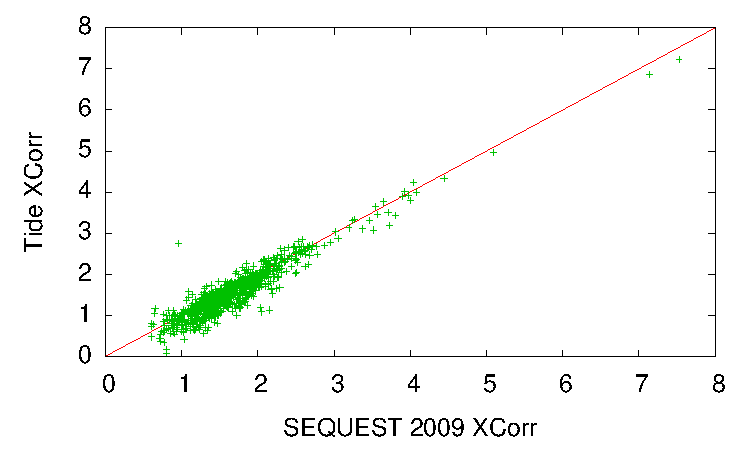
\includegraphics[width=3in]{scatter/xcorr_xcorr_worm_seqrecent_tide.pdf} \\
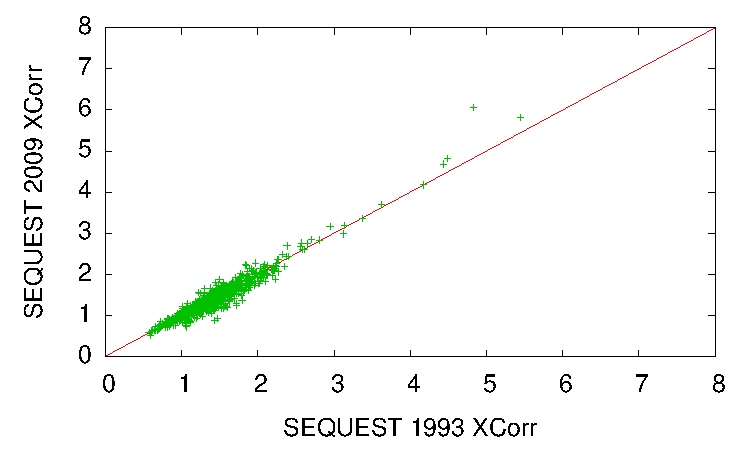
\includegraphics[width=3in]{scatter/xcorr_xcorr_yeast_seqorig_seqrecent.pdf} &
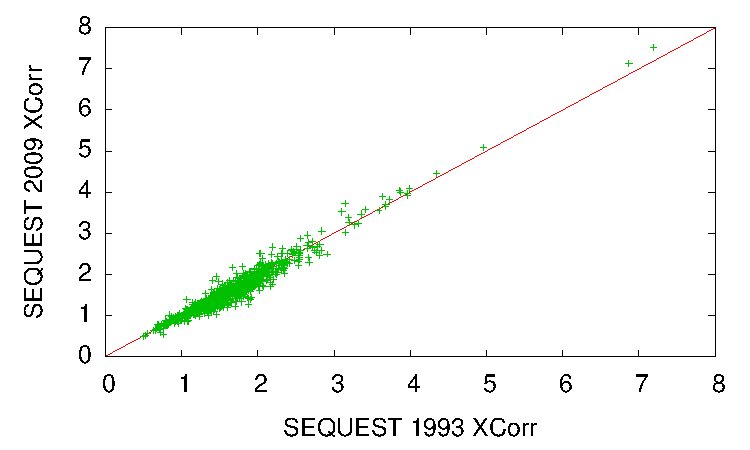
\includegraphics[width=3in]{scatter/xcorr_xcorr_worm_seqorig_seqrecent.pdf} \\
\end{tabular}
\caption{{\bf Comparison of \XCorr scores from Tide and from two
    versions of SEQUEST.}  From two different data sets (yeast and worm), 100
    spectra were selected at random for analysis by SEQUEST and by Tide.
    Searches were performed using a database of tryptic peptides from the
    corresponding organism, allowing up to two phosphorylations per peptide at
    occurrences of STY. The figure includes the top five PSMs per spectrum, as
    reported by SEQUEST.  For each PSM, we plot the SEQUEST \XCorr versus the
    \XCorr computed by Tide. In the case of the bottom figures, we plot the
    SEQUEST 1993 \XCorr scores against those computed by SEQUEST 2009.
  \label{figure:scatter}}
\end{figure}

Figure~\ref{figure:perf-chart-mods} shows the results of timing
experiments comparing Tide to the same two versions of SEQUEST when
modified peptides are included in the search. The
benchmark sets the worm and yeast data sets, each with
a $\pm 3.0$~Da mass tolerance window including fully-tryptic
peptides. Modified versions of each peptide were considered in this
experiment, with up to two phosphorylations ($+80$ Da) per peptide at
occurrences of serine, threonine, or tyrosine. In these experiments,
Tide's relative speed is an average of over 708-fold over SEQUEST and
253-fold over the indexed version of SEQUEST.

\section{Discussion}

In this work, we have described a software implementation of the
SEQUEST algorithm that searches at a rate of hundreds of spectra per
second on a single CPU.  This software thus represents more than a
thousandfold improvement in speed relative to a recent single-CPU
version of SEQUEST.

We have not directly compared Tide against the commercial indexed
version of SEQUEST, TurboSEQUEST \cite{lundgren:protein}.  This is
primarily because SEQUEST was implemented and validated on a Linux
platform, whereas TurboSEQUEST is only available running under
Windows.  However, we have shown comparisons to an indexed version of
SEQUEST that runs under Linux but is not widely available.
Furthermore, Crux was previously compared to TurboSEQUEST, and the two
programs were demonstrated to operate at approximately the same speed
\cite{park:rapid}. Thus, the results shown in
Table~\ref{figure:perf-chart} suggest that Tide, when ported to Windows,
will perform significantly faster than TurboSEQUEST.

Likewise, we have not compared Tide's speed with the speed of the full
gamut of competing database search tools, except for X!Tandem and
OMSSA as two illustrative examples.  This is because the focus of this
work is efficiency, subject to the constraint that Tide remains
faithful to the SEQUEST method. X!Tandem, OMSSA and other database
search tools do not follow the SEQUEST scoring method. To compare
different search algorithms in a reasonable fashion would require
jointly considering both efficiency and accuracy.  Accurate
identification requires not just a database search tool, but also one
or more post-processing steps that integrate information across the
entire mass spectrometry experiment, taking into account information
about the spectra, peptides and proteins.  Therefore, the most useful
comparison of search speed and accuracy should be performed at the
level of a complete identification pipeline.  Such an evaluation is
beyond the scope of the current study.

The speed improvements introduced in Tide are especially effective in
common input cases but are less dramatic in some contexts.  Shotgun
proteomics experiments commonly require enzymatic digestion of the
sample. In searching for enzymatic peptides, Tide performs up to
thousands of times faster than SEQUEST. In the non-enzymatic case Tide
is only about 7--8 times faster than the recent SEQUEST version as
tested---a far more modest gain. However, Tide was not specifically
optimized for this setting, and other opportunities for improving
Tide's algorithm might exist.

For larger peptide databases, Tide's computation time per spectrum
grows linearly in the size of the peptide database. This is because
Tide evaluates all candidate peptides against each spectrum. Larger
databases will yield proportionately larger sets of candidate peptides
and will take proportionately longer to compute, under the same
settings. The worm benchmark consists of 27,499 proteins, comparable
to the number of proteins in the human genome, although consideration
of protein isoforms in human would yield more peptides.

Most of Tide's optimizations are most effective in cases where there
are many candidate peptides per spectrum, because such cases provide
opportunities to reuse the results of earlier computations. The number
of candidates per spectrum will generally increase with the scale of
the search problem: larger protein database, wider
precursor tolerance, decreased enzyme specificity, and the inclusion
of post-translational modifications in the database. With
problems of greater scale, speed becomes increasingly important,
and Tide's results are particularly encouraging in this context.

%\subsection{Differences among SEQUEST, Crux, and Tide}

Tide's precise fidelity to Crux's scoring introduced constraints on
the approach to optimization that would not have existed had Tide's
output been allowed to vary slightly from Crux's. On the other hand,
Crux's output is less faithful to SEQUEST's output. Minor scoring
differences arise even among various versions of SEQUEST
(Figure~\ref{figure:scatter}), and were shown \cite{park:rapid} to
have little overall effect on accuracy. An informal investigation
showed that the small differences between Crux and SEQUEST were mostly
due to minor bugs in one or the other program, and that such
differences have no impact on Tide's speed.

Perhaps the greatest operational difference between Tide and SEQUEST
is that Tide does not compute SEQUEST's preliminary scoring function,
\Sp. The \Sp score was introduced into SEQUEST to speed up computation
\cite{eng:approach}.
%For each observed spectrum, SEQUEST first finds the
%top 500 peptide-spectrum matches (PSMs) by \Sp score, followed by a
%slower \XCorr computation of those 500 PSMs. The expectation is that
%\Sp will be a good enough approximation of \XCorr so that the top
%\XCorr result across all PSMs will be present among the top 500 \Sp
%scores.

However, Tide is fast enough that it can efficiently compute the full
\XCorr calculation for all PSMs and does not require (nor is it likely
to benefit greatly from) a preliminary scoring pass using \Sp.
Consequently, whereas SEQUEST may miss a candidate peptide with the
highest \XCorr because of the \Sp screen, Tide does not have this
limitation.

Note that, in some contexts \cite{anderson:new, keller:empirical,
kall:semi-supervised}, the \Sp value is needed for the top few PSMs as
an additional scoring signal. Though \Sp, which is computationally
simpler than \XCorr, is not currently included in Tide, the cost of
calculating \Sp for the top few PSMs is marginal.

%\subsection{Impact}

Most of Tide's improvements are highly optimized for \XCorr only and
are not likely to be applicable to scoring methods used in other
peptide identification software programs. On the other hand, some
optimizations included in Tide, such as the compact index, the
rolling-window join, and storing exceptional cases to disk, 
will generalize to any type of database searching. But
the specific methods for reducing the number of multiplications and
memory lookup operations, caching partial results, grouping related
theoretical peaks, on-the-fly compiling of the dot-product code, and
the like, are highly specific to the \XCorr method.

Because running SEQUEST is computationally intensive, Tide offers the
possibility to run analyses that heretofore have been prohibitively
expensive. Thus, Tide creates the potential for smaller laboratories
to conduct more sophisticated experiments, to sidestep purchasing and
managing large computing clusters, and to keep a spectrometer running
full-time when analysis would otherwise be a bottleneck. Tide also
opens the possibility of full peptide database search in real time, as
spectra are acquired by the instrument. Fast software also creates
opportunities for further improvements of the identification methods
themselves. By analyzing larger datasets, researchers can gather more
data and, in turn, devise better analytical methods.


\section*{Acknowledgments}

The authors wish to thank Charles Grant, Barbara Frewen, Larry Ruzzo,
Jimmy Eng, and Mike MacCoss for useful conversations, and Sean
McIlwain for help in the design of the benchmarking scripts used to
track running times of program runs. This work was supported by NIH
awards R01~EB007057 and T32~HG00035.

\section*{Supporting Information Available}

This material is available free of charge via the Internet at
\url{http://pubs.acs.org}.

\bibliographystyle{unsrt}
\bibliography{refs}

\clearpage
% 70 words maximum
\section*{Table of Contents Synopsis}

% Include figure (smaller than 9.0cm wide and 5.0 cm tall)
\centerline{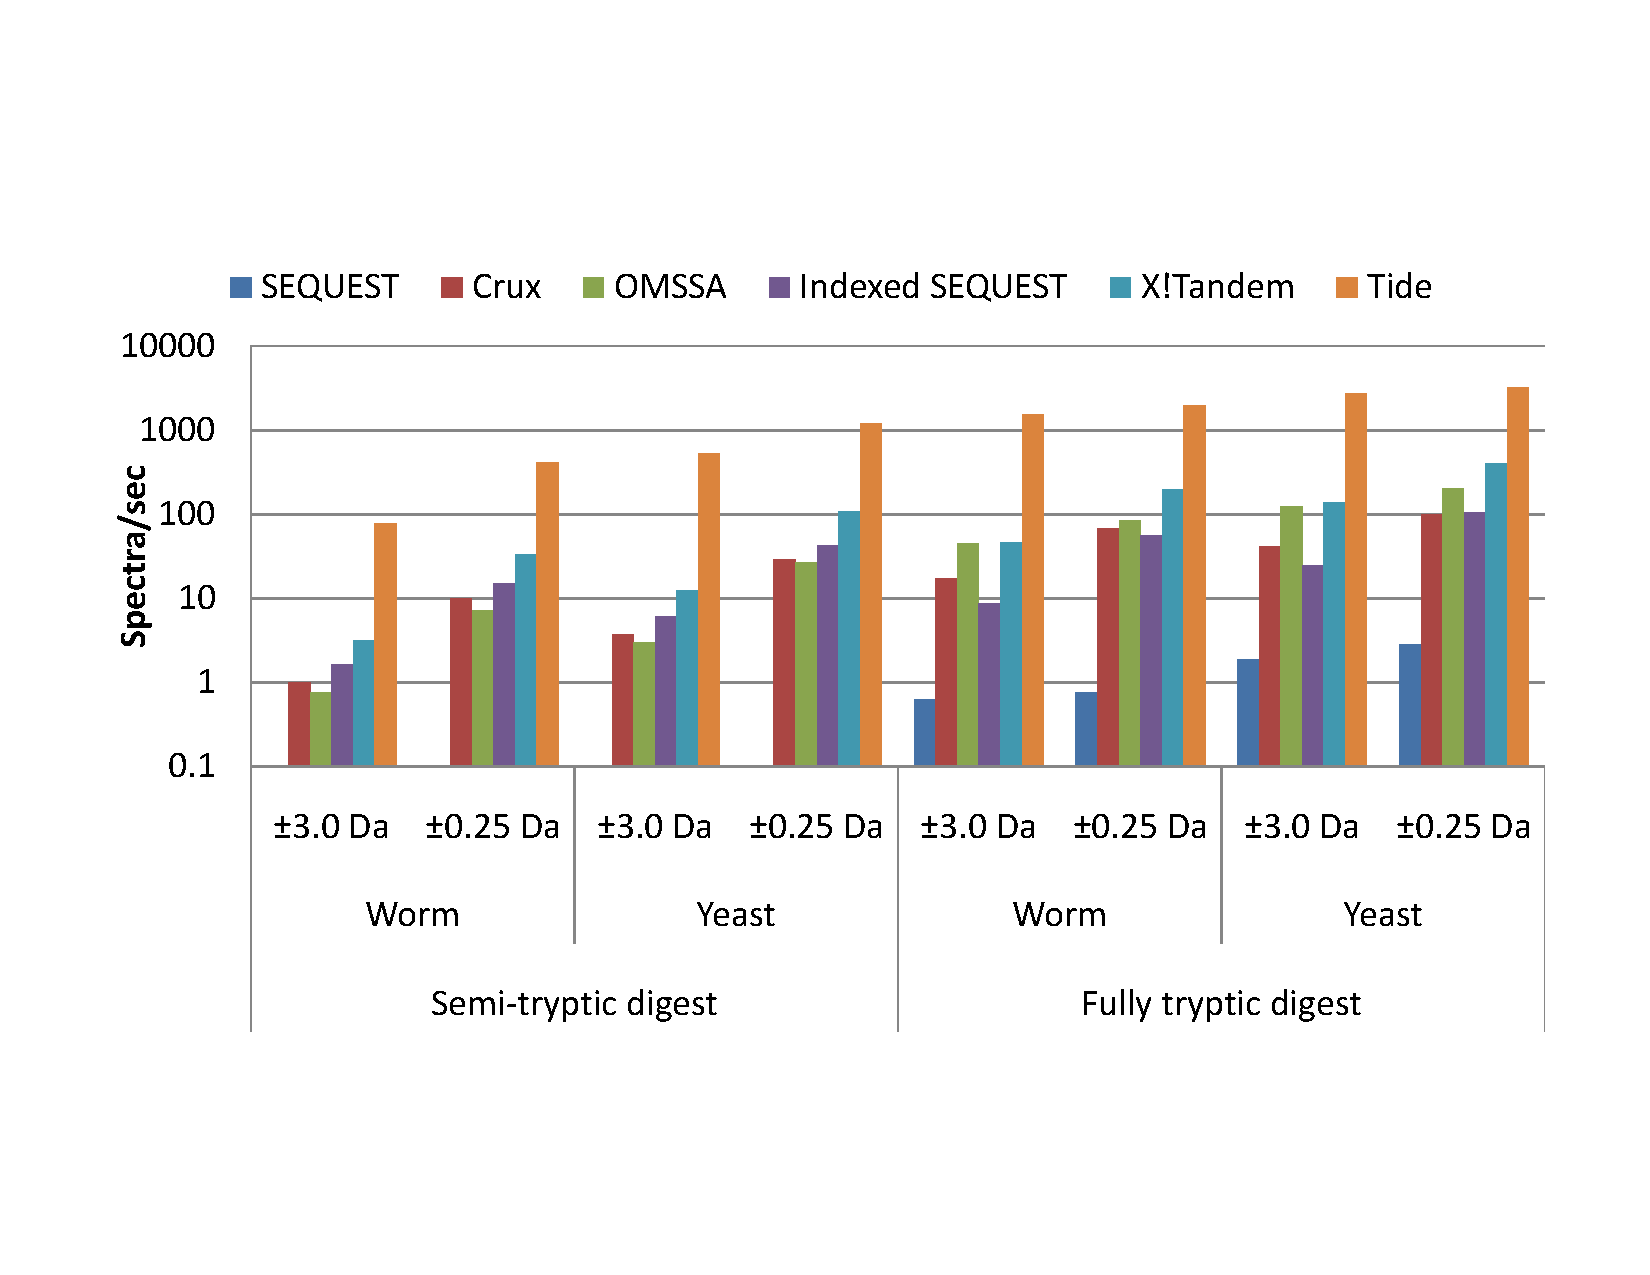
\includegraphics[width=9.0cm]{timing_chart_tocs-cropped.pdf}}

Computational analysis of mass spectra remains the bottleneck in many
proteomics experiments. We introduce Tide, which implements the
SEQUEST algorithm for peptide identification while achieving a
dramatic speedup over Crux and SEQUEST.  For example, on a single CPU,
Tide searches against a tryptic database of 27,499 proteins at a rate
of 1,550 spectra/s, which compares favorably with a rate of 8.8
spectra/s for a recent version of SEQUEST with index.

\end{document}
